% Options for packages loaded elsewhere
\PassOptionsToPackage{unicode}{hyperref}
\PassOptionsToPackage{hyphens}{url}
\documentclass[
]{article}
\usepackage{xcolor}
\usepackage[margin=1in]{geometry}
\usepackage{amsmath,amssymb}
\setcounter{secnumdepth}{-\maxdimen} % remove section numbering
\usepackage{iftex}
\ifPDFTeX
  \usepackage[T1]{fontenc}
  \usepackage[utf8]{inputenc}
  \usepackage{textcomp} % provide euro and other symbols
\else % if luatex or xetex
  \usepackage{unicode-math} % this also loads fontspec
  \defaultfontfeatures{Scale=MatchLowercase}
  \defaultfontfeatures[\rmfamily]{Ligatures=TeX,Scale=1}
\fi
\usepackage{lmodern}
\ifPDFTeX\else
  % xetex/luatex font selection
\fi
% Use upquote if available, for straight quotes in verbatim environments
\IfFileExists{upquote.sty}{\usepackage{upquote}}{}
\IfFileExists{microtype.sty}{% use microtype if available
  \usepackage[]{microtype}
  \UseMicrotypeSet[protrusion]{basicmath} % disable protrusion for tt fonts
}{}
\makeatletter
\@ifundefined{KOMAClassName}{% if non-KOMA class
  \IfFileExists{parskip.sty}{%
    \usepackage{parskip}
  }{% else
    \setlength{\parindent}{0pt}
    \setlength{\parskip}{6pt plus 2pt minus 1pt}}
}{% if KOMA class
  \KOMAoptions{parskip=half}}
\makeatother
\usepackage{longtable,booktabs,array}
\usepackage{calc} % for calculating minipage widths
% Correct order of tables after \paragraph or \subparagraph
\usepackage{etoolbox}
\makeatletter
\patchcmd\longtable{\par}{\if@noskipsec\mbox{}\fi\par}{}{}
\makeatother
% Allow footnotes in longtable head/foot
\IfFileExists{footnotehyper.sty}{\usepackage{footnotehyper}}{\usepackage{footnote}}
\makesavenoteenv{longtable}
\usepackage{graphicx}
\makeatletter
\newsavebox\pandoc@box
\newcommand*\pandocbounded[1]{% scales image to fit in text height/width
  \sbox\pandoc@box{#1}%
  \Gscale@div\@tempa{\textheight}{\dimexpr\ht\pandoc@box+\dp\pandoc@box\relax}%
  \Gscale@div\@tempb{\linewidth}{\wd\pandoc@box}%
  \ifdim\@tempb\p@<\@tempa\p@\let\@tempa\@tempb\fi% select the smaller of both
  \ifdim\@tempa\p@<\p@\scalebox{\@tempa}{\usebox\pandoc@box}%
  \else\usebox{\pandoc@box}%
  \fi%
}
% Set default figure placement to htbp
\def\fps@figure{htbp}
\makeatother
\setlength{\emergencystretch}{3em} % prevent overfull lines
\providecommand{\tightlist}{%
  \setlength{\itemsep}{0pt}\setlength{\parskip}{0pt}}
\usepackage{float}
\usepackage{booktabs}
\usepackage{longtable}
\usepackage{array}
\usepackage{multirow}
\usepackage{wrapfig}
\usepackage{colortbl}
\usepackage{pdflscape}
\usepackage{tabu}
\usepackage{threeparttable}
\usepackage{threeparttablex}
\usepackage[normalem]{ulem}
\usepackage{makecell}
\usepackage{xcolor}
\usepackage{bookmark}
\IfFileExists{xurl.sty}{\usepackage{xurl}}{} % add URL line breaks if available
\urlstyle{same}
\hypersetup{
  pdftitle={Technical Execution Roadmap --- Full Project Report},
  pdfauthor={Colombini Francesco \& Hosen Jabed},
  hidelinks,
  pdfcreator={LaTeX via pandoc}}

\title{Technical Execution Roadmap --- Full Project Report}
\usepackage{etoolbox}
\makeatletter
\providecommand{\subtitle}[1]{% add subtitle to \maketitle
  \apptocmd{\@title}{\par {\large #1 \par}}{}{}
}
\makeatother
\subtitle{Sentiment Analysis Project \textbar{} JEMIB IT\&BI Area ·
Spring 2026}
\author{Colombini Francesco \& Hosen Jabed}
\date{May 01, 2026}

\begin{document}
\maketitle

{
\setcounter{tocdepth}{4}
\tableofcontents
}
\begin{center}\rule{0.5\linewidth}{0.5pt}\end{center}

\begin{center}\rule{0.5\linewidth}{0.5pt}\end{center}

\section{Step 1 --- Data Ingestion \& Schema
Validation}\label{step-1-data-ingestion-schema-validation}

Both CSVs were loaded with \texttt{read\_csv2()} (semicolon-delimited
format), and the schema was immediately verified against the project
specification. Loading data without inspecting its structure first is
the most common source of silent analytical errors, a miscast column
type will corrupt every downstream calculation without throwing a single
error message.

The table below maps each column to its expected type and valid range.
Any deviation from this contract (e.g.~\texttt{Year} read as
\texttt{character}) must be corrected before proceeding.

\begin{longtable}[t]{llll}
\caption{\label{tab:schema-table}Schema Reference Table — Training Set}\\
\toprule
Column & Type & Expected\_Range & Phase\_1\_Role\\
\midrule
Year & int & 2010–2023 & temporal trend\\
Month & int & 1–12 & seasonality\\
Day & int & 1–31 & granularity\\
date & Date & derived & timeline axis\\
time\_of\_tweet & factor(3) & morning/noon/night & posting rhythm\\
\addlinespace
text & chr & free text & NLP corpus\\
sentiment & factor(3) & neg/neu/pos & target variable\\
platform & factor(3) & FB/IG/TW & stratification variable\\
\bottomrule
\end{longtable}

\begin{verbatim}
## Train set — post-schema enforcement:
\end{verbatim}

\begin{verbatim}
##       Year          Month             Day             date           
##  Min.   :2010   Min.   : 1.000   Min.   : 1.00   Min.   :2010-11-12  
##  1st Qu.:2018   1st Qu.: 2.000   1st Qu.: 8.00   1st Qu.:2018-08-31  
##  Median :2020   Median : 5.000   Median :17.00   Median :2020-08-24  
##  Mean   :2020   Mean   : 5.714   Mean   :16.08   Mean   :2020-05-03  
##  3rd Qu.:2023   3rd Qu.: 9.000   3rd Qu.:23.00   3rd Qu.:2023-01-18  
##  Max.   :2023   Max.   :12.000   Max.   :31.00   Max.   :2023-05-30  
##  Time of Tweet     text              sentiment        Platform  
##  morning:140   Length:420         negative:115   Facebook :140  
##  noon   :144   Class :character   neutral :167   Instagram:144  
##  night  :136   Mode  :character   positive:138   Twitter  :136  
##                                                                 
##                                                                 
## 
\end{verbatim}

\begin{center}\rule{0.5\linewidth}{0.5pt}\end{center}

\section{Step 2 --- Structural Data Quality
Audit}\label{step-2-structural-data-quality-audit}

Before any analysis, the dataset must pass a formal quality audit. This
is not a formality, it is the statistical foundation that justifies
every cleaning decision documented in Step 3. Any missing values,
duplicate posts, or temporal anomalies detected here are flagged,
quantified, and handled transparently so that conclusions drawn from the
data are defensible.

\subsection{2.1 Missing Value Audit}\label{missing-value-audit}

A missing value in \texttt{sentiment} would silently exclude a post from
class-distribution analysis. A missing \texttt{date} would corrupt the
temporal trend chart. The table below confirms whether any column
contains \texttt{NA} values and at what rate.

\begin{longtable}[t]{lrr}
\caption{\label{tab:data-quality}Missing Value Audit — Training Set}\\
\toprule
column & n\_missing & pct\_missing\\
\midrule
Year & 0 & 0\\
Month & 0 & 0\\
Day & 0 & 0\\
date & 0 & 0\\
Time of Tweet & 0 & 0\\
\addlinespace
text & 0 & 0\\
sentiment & 0 & 0\\
Platform & 0 & 0\\
\bottomrule
\end{longtable}

\subsection{2.2 Duplicate Detection \&
Removal}\label{duplicate-detection-removal}

Duplicate posts --- the same text appearing more than once --- inflate
word frequency counts and bias the sentiment distribution. They most
commonly arise from cross-platform reposts (the same message published
on both Facebook and Instagram). We key deduplication on \texttt{text}
alone: the same linguistic content seen twice carries the same NLP
signal regardless of which platform it appeared on, so only the first
occurrence is retained.

\begin{verbatim}
## Rows after deduplication: 326 | Rows removed: 94
\end{verbatim}

\begin{longtable}[t]{lr}
\caption{\label{tab:duplicates}Short-Post Flag Audit (< 3 words)}\\
\toprule
flag\_short & n\\
\midrule
FALSE & 309\\
TRUE & 17\\
\bottomrule
\end{longtable}

\subsection{2.3 Temporal Integrity
Check}\label{temporal-integrity-check}

The research question covers a decade of social media data, so if the
date range is narrower than expected, or if any dates are invalid (e.g.
February 30), the temporal trend analysis in Step 6 would be silently
misleading. For this reason a temporal integrity check was inspected.
The table below reports the earliest and the latest posts.

\begin{longtable}[t]{llrr}
\caption{\label{tab:date-validation}Temporal Integrity Check}\\
\toprule
earliest\_post & latest\_post & n\_years & n\_invalid\_dates\\
\midrule
2010-11-12 & 2023-05-30 & 14 & 0\\
\bottomrule
\end{longtable}

\begin{center}\rule{0.5\linewidth}{0.5pt}\end{center}

\section{Step 3 --- Text Cleaning \& Preprocessing
Pipeline}\label{step-3-text-cleaning-preprocessing-pipeline}

Social media language is structurally adversarial to standard NLP tools.
URLs are pure noise with zero semantic content. Emojis encode emotion
but are invisible to word-frequency counters. Contractions (``can't'',
``I'll'') fragment token counts by treating the same concept as multiple
distinct strings. Each transformation below addresses one specific
failure mode. The raw text is always preserved in \texttt{text\_raw} so
that every cleaning decision can be challenged, reversed, or re-run
without reloading the original CSV.

\subsection{3.1 Character-Level
Normalisation}\label{character-level-normalisation}

\begin{table}[!h]
\centering
\caption{\label{tab:text-cleaning-pipeline}Cleaning Pipeline — Before vs After (sample)}
\centering
\fontsize{10}{12}\selectfont
\begin{tabular}[t]{>{\raggedright\arraybackslash}p{6cm}>{\raggedright\arraybackslash}p{6cm}}
\toprule
\textbf{text\_raw} & \textbf{text}\\
\midrule
so no rice or crusty bread with the chili .. aawww & so no rice or crusty bread with the chili aawww\\
\_x\_atl you mean jack barakat`s?! wow so have you ever
gone to his house? hehe i mean your ssoo lucky to have the
address! & xatl you mean jack barakats wow so have you ever gone to his
house hehe i mean your ssoo lucky to have the address\\
really great football match & really great football match\\
\bottomrule
\end{tabular}
\end{table}

\subsection{3.2 Tokenisation, Stop-word Removal \&
Stemming}\label{tokenisation-stop-word-removal-stemming}

Tokenisation is the pivot point of the entire NLP pipeline, it
transforms the dataset from a table of documents into a table of
individual words. Once tokenised, two further transformations are
applied:

\begin{itemize}
\tightlist
\item
  \textbf{Stop-word removal:} Eliminating words like ``the'', ``is'',
  ``and'' that appear in every sentiment class with equal frequency and
  therefore carry no discriminative signal.
\item
  \textbf{Stemming:} Collapsing inflected forms (``running'', ``runs'',
  ``ran'') to a shared root (``run'') so that related word forms are
  counted together rather than separately.
\end{itemize}

\begin{verbatim}
## Total tokens after cleaning: 1900
\end{verbatim}

\begin{verbatim}
## Unique stems: 987
\end{verbatim}

\begin{center}\rule{0.5\linewidth}{0.5pt}\end{center}

\section{Step 4 --- Univariate EDA: Sentiment
Distribution}\label{step-4-univariate-eda-sentiment-distribution}

The first question any analyst must answer about a classification
dataset is: \textbf{are the classes balanced?} Class imbalance is not
only a modelling concern --- it distorts the story told in the
dashboard. If 40\% of posts are neutral and a bar chart displays
equal-height bars, the chart is actively misleading the reader. This
step quantifies the imbalance and provides the statistical evidence to
characterise it accurately in the report.

\subsection{4.1 Frequency Table}\label{frequency-table}

\begin{longtable}[t]{lrl}
\caption{\label{tab:sentiment-dist}Sentiment Class Distribution — Training Set (n = 326)}\\
\toprule
sentiment & n & percent\\
\midrule
negative & 93 & 28.5\%\\
neutral & 126 & 38.7\%\\
positive & 107 & 32.8\%\\
\bottomrule
\end{longtable}

\subsection{4.2 Chi-Square Goodness-of-Fit
Test}\label{chi-square-goodness-of-fit-test}

A bar chart alone cannot confirm whether the observed class proportions
represent a statistically meaningful deviation from balance. The
chi-square goodness-of-fit test formalises this question: under the null
hypothesis, each of the three sentiment classes contains exactly 1/3 of
all posts. A significant result (p \textless{} 0.05) means the observed
distribution is unlikely to have arisen by chance alone.

\begin{verbatim}
## Chi-square test for class balance:
\end{verbatim}

\begin{verbatim}
##   $\chi^2$(2) = 5.049
\end{verbatim}

\begin{verbatim}
##   p-value = 0.0801
\end{verbatim}

\begin{verbatim}
##   Interpretation: No significant deviation from uniform distribution detected at alfa = 0.05.
\end{verbatim}

The p-value of \textbf{0.08 sits above the conventional alfa = 0.05
threshold}, so we formally fail to reject the null hypothesis of
balance. However, this is a \textbf{borderline result} that deserves
honest reporting: with only 326 posts after deduplication, the test has
limited statistical power. The descriptive picture, neutral at
\textasciitilde38.7\% versus negative at \textasciitilde28.5\%, reveals
a mild practical imbalance that will be relevant context for any
accuracy metric computed in next phase.

\subsection{4.3 Bar Chart}\label{bar-chart}

\begin{figure}[H]

{\centering 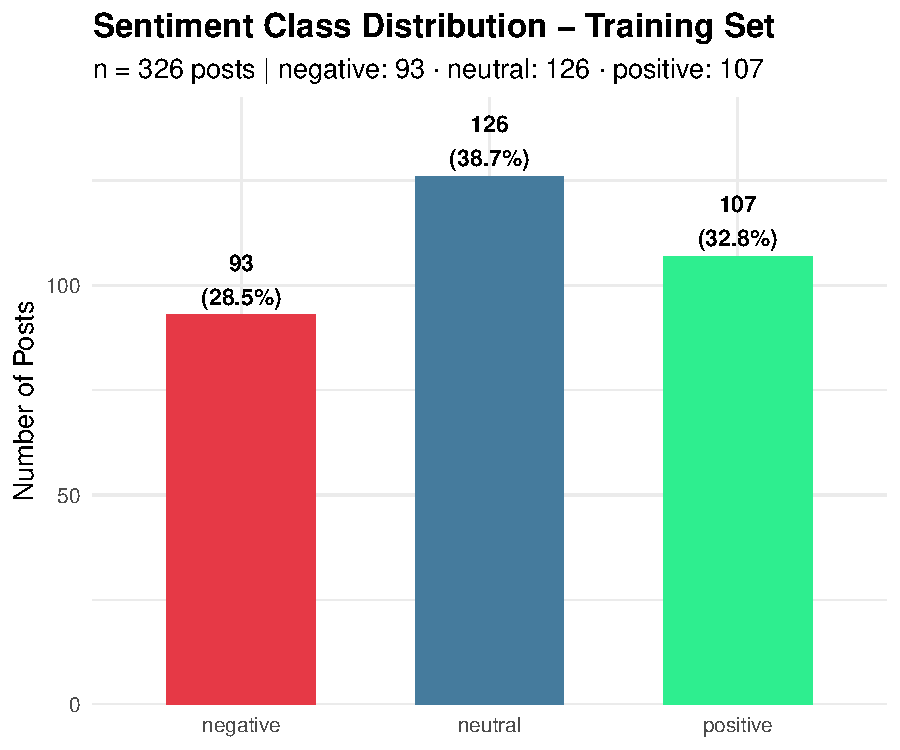
\includegraphics{Full_Project_Report_files/figure-latex/sentiment-bar-1} 

}

\caption{Figure 1: Sentiment Class Distribution}\label{fig:sentiment-bar}
\end{figure}

\begin{center}\rule{0.5\linewidth}{0.5pt}\end{center}

\section{Step 5 --- Bivariate EDA}\label{step-5-bivariate-eda}

Bivariate analysis moves beyond describing individual variables to
asking whether two variables are \textbf{associated} with each other.
Both associations tested below (platform and posting time) are evaluated
with chi-square tests and supplemented with an effect size metric,
because a statistically significant result in a small dataset does not
necessarily imply a practically meaningful relationship.

\subsection{\texorpdfstring{5.1 Sentiment \(\times\)
Platform}{5.1 Sentiment \textbackslash times Platform}}\label{sentiment-times-platform}

The structural affordances of each platform, Facebook's long-form posts,
Instagram's caption-driven visual format, and Twitter's
character-limited microblog, plausibly shape the language users employ,
and therefore the sentiment that language expresses. This hypothesis is
tested formally rather than assumed, because the platform filter in the
dashboard should only be presented as analytically meaningful if the
data supports it.

\begin{longtable}[t]{llll}
\caption{\label{tab:sentiment-platform}Sentiment Distribution by Platform (row \%)}\\
\toprule
Platform & negative & neutral & positive\\
\midrule
Facebook & 30.8\% (32) & 34.6\% (36) & 34.6\% (36)\\
Instagram & 31.6\% (36) & 36.8\% (42) & 31.6\% (36)\\
Twitter & 23.1\% (25) & 44.4\% (48) & 32.4\% (35)\\
\bottomrule
\end{longtable}

\begin{verbatim}
## Platform vs Sentiment association:
\end{verbatim}

\begin{verbatim}
##  - Chi-squared ( 4 ) = 3.285
\end{verbatim}

\begin{verbatim}
##  - P-value  = 0.5114
\end{verbatim}

\begin{verbatim}
##  - Cramér's V = 0.071  - Effect size: negligible
\end{verbatim}

With Chi-squared = 3.285, p = 0.51, and Cramér's V = 0.071, \textbf{the
data provide no evidence of an association between platform and
sentiment}. The sentiment composition observed across Facebook,
Instagram and Twitter is fully consistent with random variation. This is
itself a finding: it tells Emma Martin that the \emph{medium does not
shapethe emotional message} in this dataset, and it means that platform
should not be presented as a meaningful driver of sentiment in the
dashboard.

\begin{figure}[H]

{\centering 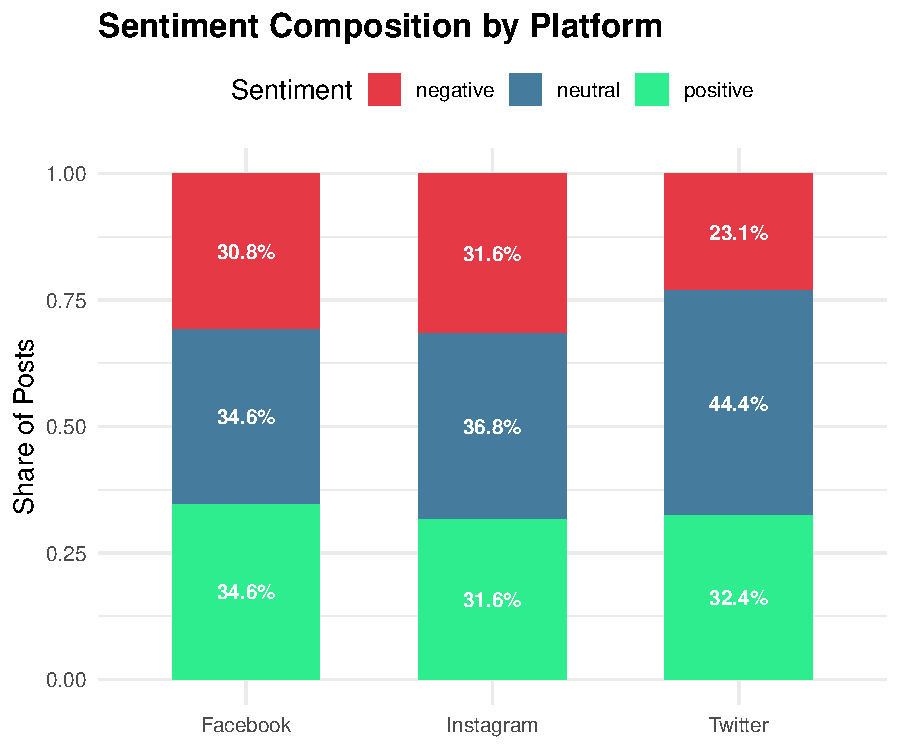
\includegraphics{Full_Project_Report_files/figure-latex/sentiment-platform-plot-1} 

}

\caption{Figure 2: Sentiment Composition by Platform}\label{fig:sentiment-platform-plot}
\end{figure}

\begin{center}\rule{0.5\linewidth}{0.5pt}\end{center}

\subsection{\texorpdfstring{5.2 Sentiment \(\times\) Time of
Tweet}{5.2 Sentiment \textbackslash times Time of Tweet}}\label{sentiment-times-time-of-tweet}

Posting time is a behavioural proxy for emotional state. Morning posts
may reflect aspirational or goal-setting framing; night posts are more
likely to capture emotional discharge after the events of the day --- a
pattern well-documented in mass-psychology literature. This analysis
tests whether this hypothesis holds in the current dataset, providing
Emma Martin with time-of-day granularity for her research conclusions.

\begin{longtable}[t]{llll}
\caption{\label{tab:sentiment-time}Sentiment Distribution by Time of Tweet (row \%)}\\
\toprule
Time of Tweet & negative & neutral & positive\\
\midrule
morning & 30.8\% (33) & 39.3\% (42) & 29.9\% (32)\\
noon & 24.5\% (27) & 41.8\% (46) & 33.6\% (37)\\
night & 30.3\% (33) & 34.9\% (38) & 34.9\% (38)\\
\bottomrule
\end{longtable}

\begin{figure}[H]

{\centering 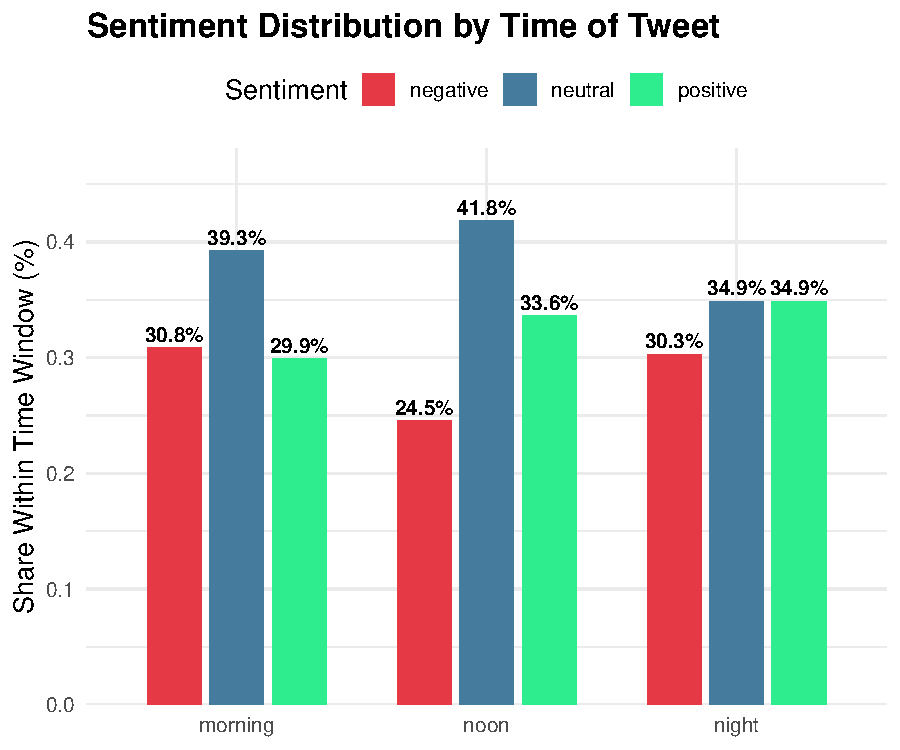
\includegraphics{Full_Project_Report_files/figure-latex/time-plot-1} 

}

\caption{Figure 3: Sentiment Distribution by Time of Tweet}\label{fig:time-plot}
\end{figure}

\begin{center}\rule{0.5\linewidth}{0.5pt}\end{center}

\section{Step 6 --- Temporal EDA: Historical Sentiment Trend
(2010--2023)}\label{step-6-temporal-eda-historical-sentiment-trend-20102023}

This is the the client's core research question, \emph{``how has
sentiment on social networks evolved overthe last decade?''}, is
answered directly here. \textbf{Proportions} are plotted rather than raw
counts to correct for the unequal number of posts per year: a year with
5 posts and a year with 50 posts are not directly comparable on a
raw-count axis.

The point size encodes the post volume per year, allowing readers to
discount years with very few observations (where proportion estimates
are noisy) without needing to consult a separate table.

\subsection{6.1 Annual Trend Lines}\label{annual-trend-lines}

\begin{figure}[H]

{\centering 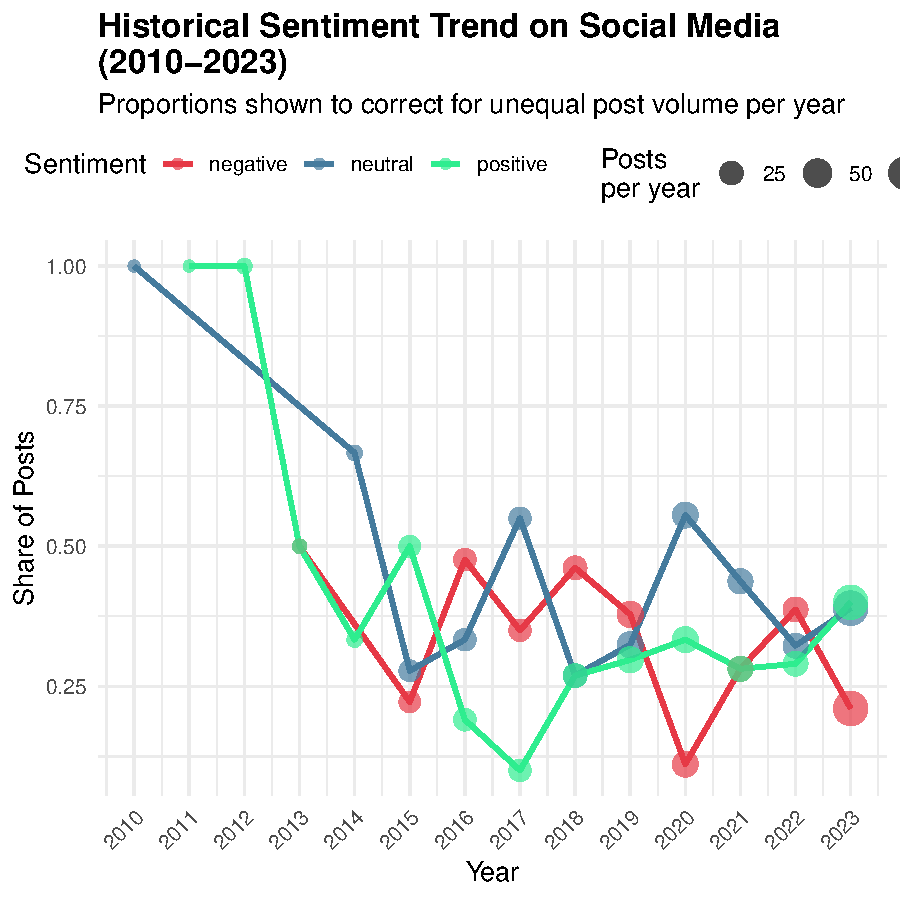
\includegraphics{Full_Project_Report_files/figure-latex/yearly-trend-1} 

}

\caption{Figure 4: Historical Sentiment Trend (2010–2023)}\label{fig:yearly-trend}
\end{figure}

\subsection{6.2 Monthly Seasonality
Heatmap}\label{monthly-seasonality-heatmap}

Beyond the annual trend, Emma Martin's research may benefit from
understanding \textbf{within-year seasonality} --- whether positive
sentiment concentrates in specific months. The heatmap below shows the
share of positive posts by month and platform, revealing any seasonal
patterns that the annual trend lines cannot capture.

\begin{figure}[H]

{\centering 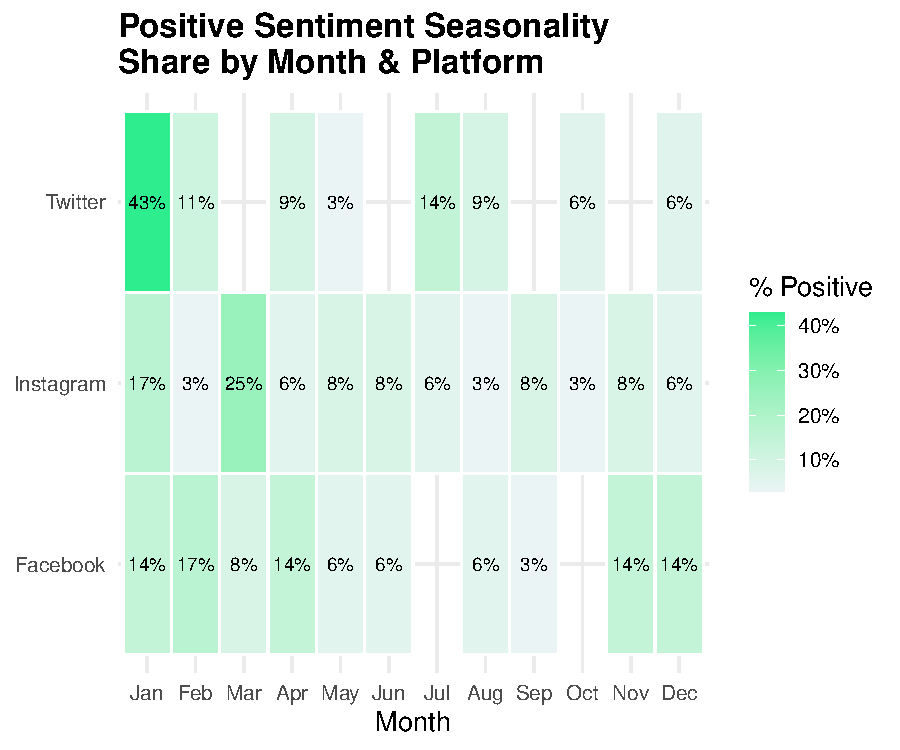
\includegraphics{Full_Project_Report_files/figure-latex/monthly-heatmap-1} 

}

\caption{Figure 5: Positive Sentiment Seasonality Heatmap}\label{fig:monthly-heatmap}
\end{figure}

\begin{center}\rule{0.5\linewidth}{0.5pt}\end{center}

\section{Step 7 --- Cleaned Dataset
Export}\label{step-7-cleaned-dataset-export}

The cleaned, tokenised training dataset is exported here as the
\textbf{single source of truth} for Phase 2 (modelling) and Phase 3
(dashboard). Separating the cleaned artefacts from the raw CSVs enforces
a clean handoff: Phase 2 picks up from \texttt{SA\_train\_cleaned.csv}
without re-running or re-interpreting any preprocessing step, and the
pipeline remains fully auditable end-to-end.

\begin{verbatim}
## Export complete:
\end{verbatim}

\begin{verbatim}
##   SA_train_cleaned.csv — 326 rows $  imes$ 11 columns
\end{verbatim}

\begin{verbatim}
##   SA_train_tokens.csv        — 1900 token rows
\end{verbatim}

\begin{center}\rule{0.5\linewidth}{0.5pt}\end{center}

\section{Step 8 --- Test Set Cleaning \& Quality
Audit}\label{step-8-test-set-cleaning-quality-audit}

The test set (\texttt{SA\_test}) receives the \textbf{identical cleaning
pipeline} applied to the training set in Steps 1--3, with one structural
difference: it carries no \texttt{sentiment} column, because it is the
unlabelled batch that the algorithm will classify each month. Every
other transformation, type enforcement, deduplication, text
normalisation, tokenisation, is applied in the same order and with the
same parameters to guarantee that the two datasets share an identical
linguistic representation when the model is applied.

\subsection{8.1 Schema Enforcement}\label{schema-enforcement}

\begin{verbatim}
## Test set — post-schema enforcement:
\end{verbatim}

\begin{verbatim}
##       Year          Month             Day             date           
##  Min.   :2023   Min.   : 6.000   Min.   : 1.00   Min.   :2023-06-01  
##  1st Qu.:2023   1st Qu.: 7.000   1st Qu.: 7.00   1st Qu.:2023-07-06  
##  Median :2023   Median : 8.000   Median :14.00   Median :2023-08-24  
##  Mean   :2023   Mean   : 8.051   Mean   :13.66   Mean   :2023-08-14  
##  3rd Qu.:2023   3rd Qu.: 9.000   3rd Qu.:20.00   3rd Qu.:2023-09-16  
##  Max.   :2023   Max.   :10.000   Max.   :30.00   Max.   :2023-10-17  
##  NA's   :1                                       NA's   :1           
##  Time of Tweet     text           sentiment           Platform 
##  morning:31    Length:79          Mode:logical   Facebook :29  
##  noon   :23    Class :character   NA's:79        Instagram:27  
##  night  :25    Mode  :character                  Twitter  :23  
##                                                                
##                                                                
##                                                                
## 
\end{verbatim}

\subsection{8.2 Missing Value Audit}\label{missing-value-audit-1}

\begin{longtable}[t]{lrr}
\caption{\label{tab:test-missing}Missing Value Audit — Test Set}\\
\toprule
column & n\_missing & pct\_missing\\
\midrule
\cellcolor{gray!10}{Year} & \cellcolor{gray!10}{1} & \cellcolor{gray!10}{1.27}\\
Month & 0 & 0.00\\
\cellcolor{gray!10}{Day} & \cellcolor{gray!10}{0} & \cellcolor{gray!10}{0.00}\\
date & 1 & 1.27\\
\cellcolor{gray!10}{Time of Tweet} & \cellcolor{gray!10}{0} & \cellcolor{gray!10}{0.00}\\
\addlinespace
text & 0 & 0.00\\
\cellcolor{gray!10}{sentiment} & \cellcolor{gray!10}{79} & \cellcolor{gray!10}{100.00}\\
Platform & 0 & 0.00\\
\bottomrule
\end{longtable}

\subsection{8.3 Duplicate Detection \&
Removal}\label{duplicate-detection-removal-1}

\begin{verbatim}
## Test set — exact text duplicates detected: 12
\end{verbatim}

\begin{verbatim}
## Rows after deduplication: 67 | Rows removed: 12
\end{verbatim}

\begin{longtable}[t]{lr}
\caption{\label{tab:test-duplicates}Short-Post Flag Audit — Test Set (< 3 words)}\\
\toprule
flag\_short & n\\
\midrule
\cellcolor{gray!10}{FALSE} & \cellcolor{gray!10}{66}\\
TRUE & 1\\
\bottomrule
\end{longtable}

\subsection{8.4 Temporal Integrity
Check}\label{temporal-integrity-check-1}

\begin{longtable}[t]{llrr}
\caption{\label{tab:test-date-validation}Temporal Integrity Check — Test Set}\\
\toprule
earliest\_post & latest\_post & n\_years & n\_invalid\_dates\\
\midrule
2023-06-01 & 2023-10-17 & 2 & 1\\
\bottomrule
\end{longtable}

\subsection{8.5 Character-Level Text
Normalisation}\label{character-level-text-normalisation}

\begin{table}[!h]
\centering
\caption{\label{tab:test-text-cleaning}Test Set Cleaning — Before vs After (sample)}
\centering
\fontsize{10}{12}\selectfont
\begin{tabular}[t]{>{\raggedright\arraybackslash}p{6cm}>{\raggedright\arraybackslash}p{6cm}}
\toprule
\textbf{text\_raw} & \textbf{text}\\
\midrule
almost died. laptop screen was set to 100\% brightness
after i reinstalled windows vista. & almost died laptop screen was set to brightness after i
reinstalled windows vista\\
waiting for tish to get off. got to drive my moms crv
to pick her up all my myself and duckie. first time & waiting for tish to get off got to drive my moms crv to
pick her up all my myself and duckie first time\\
your attitude looks like autistics child & your attitude looks like autistics child\\
\bottomrule
\end{tabular}
\end{table}

\subsection{8.6 Tokenisation, Stop-word Removal \&
Stemming}\label{tokenisation-stop-word-removal-stemming-1}

\begin{verbatim}
## Test set — total tokens after cleaning: 428
\end{verbatim}

\begin{verbatim}
## Test set — unique stems: 278
\end{verbatim}

\subsection{8.7 Vocabulary Overlap: Train vs
Test}\label{vocabulary-overlap-train-vs-test}

\begin{longtable}[t]{lrl}
\caption{\label{tab:vocab-overlap}Vocabulary Overlap: Training vs Test Stems}\\
\toprule
Metric & Count & Share\\
\midrule
\cellcolor{gray!10}{Stems in both train \& test} & \cellcolor{gray!10}{152} & \cellcolor{gray!10}{13.7\%}\\
Stems in test only (unseen by model) & 126 & 11.3\%\\
\cellcolor{gray!10}{Stems in train only (absent from test)} & \cellcolor{gray!10}{835} & \cellcolor{gray!10}{75\%}\\
\bottomrule
\end{longtable}

A high share of test-only stems signals potential domain shift and
should be reported to the Phase 2 analyst before model deployment. A
rate below 15\% is generally considered acceptable for a same-domain
corpus.

\subsection{8.8 Test Set Export}\label{test-set-export}

\begin{verbatim}
## Test set export complete:
\end{verbatim}

\begin{verbatim}
##   SA_test_cleaned.csv  — 67 rows x 11 columns
\end{verbatim}

\begin{verbatim}
##   SA_test_tokens.csv   — 428 token rows
\end{verbatim}

\section{Step 9 --- Model Development \&
Implementation}\label{step-9-model-development-implementation}

The modeling phase involved the design, training, and optimization of
seven distinct sentiment classification architectures. This phase was
specifically engineered to handle the challenges of a relatively small
dataset while maximizing predictive power.

\subsection{9.1 Data Pipeline \&
Pre-modeling}\label{data-pipeline-pre-modeling}

Before the training loops were initiated, a robust data pipeline was
established to ensure consistency and quality.

\subsubsection{9.1.1 Advanced Data
Augmentation}\label{advanced-data-augmentation}

To mitigate the risk of overfitting on a limited sample size, we
implemented an automated text augmentation strategy.

\begin{itemize}
\tightlist
\item
  \textbf{Method:} Synonym replacement using the WordNet database.
\item
  \textbf{Logic:} For each original training sample, the
  \texttt{augment\_text\_data} function generates additional synthetic
  samples by replacing key words with their synonyms while preserving
  the original sentiment label.
\item
  \textbf{Impact:} This artificially expanded the training distribution,
  forcing the models to learn semantic meaning rather than just
  memorizing specific keyword occurrences.
\end{itemize}

\subsubsection{9.1.2 Deterministic
Reproducibility}\label{deterministic-reproducibility}

Given the sensitivity of deep learning models to random initialization,
a strict seeding protocol was enforced:

\begin{itemize}
\tightlist
\item
  \textbf{Seed Value:} \texttt{12345}
\item
  \textbf{Scope:} Applied to \texttt{random}, \texttt{numpy},
  \texttt{torch} (CPU), and \texttt{torch.cuda} (GPU).
\item
  \textbf{Function:} The \texttt{set\_seed(RANDOM\_STATE)} function was
  executed at the start of every model script to ensure that results are
  100\% reproducible across different environments.
\end{itemize}

\subsection{9.2 Model Architecture
Specifications}\label{model-architecture-specifications}

We deployed a diverse suite of models to evaluate the trade-offs between
computational complexity and classification accuracy.

\subsubsection{9.2.1 Transformer-Based Architectures (Deep
Learning)}\label{transformer-based-architectures-deep-learning}

These models utilize the self-attention mechanism to capture deep
contextual relationships within the text. 1. \textbf{RoBERTa
(roberta-base):} A robustly optimized version of BERT that was trained
on a larger corpus with longer sequences and larger batches. 2.
\textbf{BERT (bert-base-uncased):} The industry standard for
bidirectional context understanding. 3. \textbf{Multilingual BERT
(bert-base-multilingual-uncased):} Evaluated for its ability to
generalize across different linguistic styles. 4. \textbf{DistilBERT
(distilbert-base-uncased):} A smaller, faster, and lighter version of
BERT that retains approximately 97\% of its performance.

\subsubsection{9.2.2 Statistical Classifiers (Machine
Learning)}\label{statistical-classifiers-machine-learning}

These models rely on frequency-based feature extraction (TF-IDF). 5.
\textbf{Logistic Regression:} A linear model optimized using the
\texttt{liblinear} solver. 6. \textbf{Support Vector Machine (SVM):}
Implemented with a linear kernel to find the optimal separating
hyperplane in a high-dimensional TF-IDF space. 7. \textbf{Multinomial
Naive Bayes:} A probabilistic classifier based on Bayes' theorem with
the assumption of independence between features.

\subsection{9.3 Training \& Optimization
Hyperparameters}\label{training-optimization-hyperparameters}

All Transformer models were fine-tuned using a standardized
high-performance training loop:

\begin{itemize}
\tightlist
\item
  \textbf{Optimizer:} \texttt{AdamW} (Adam with Weight Decay) to prevent
  parameter divergence.
\item
  \textbf{Scheduler:} \texttt{get\_linear\_schedule\_with\_warmup} (500
  warmup steps) to stabilize the initial stages of training.
\item
  \textbf{Loss Function:} \texttt{CrossEntropyLoss} (standard for
  multi-class classification).
\item
  \textbf{Batch Size:} 16.
\item
  \textbf{Max Sequence Length:} 64 tokens.
\item
  \textbf{Learning Rate:} 1e-5.
\item
  \textbf{Weight Decay:} 0.01.
\end{itemize}

\section{Step 10 --- Technical Result Analysis \& Comparative
Evaluation}\label{step-10-technical-result-analysis-comparative-evaluation}

This section provides a granular analysis of model performance across
the holdout test set.

\subsection{10.1 Global Accuracy
Leaderboard}\label{global-accuracy-leaderboard}

The following table presents the final validated results.

\begin{longtable}[]{@{}
  >{\centering\arraybackslash}p{(\linewidth - 8\tabcolsep) * \real{0.2174}}
  >{\raggedright\arraybackslash}p{(\linewidth - 8\tabcolsep) * \real{0.1739}}
  >{\centering\arraybackslash}p{(\linewidth - 8\tabcolsep) * \real{0.2174}}
  >{\centering\arraybackslash}p{(\linewidth - 8\tabcolsep) * \real{0.2174}}
  >{\raggedright\arraybackslash}p{(\linewidth - 8\tabcolsep) * \real{0.1739}}@{}}
\toprule\noalign{}
\begin{minipage}[b]{\linewidth}\centering
Rank
\end{minipage} & \begin{minipage}[b]{\linewidth}\raggedright
Model Architecture
\end{minipage} & \begin{minipage}[b]{\linewidth}\centering
Test Accuracy
\end{minipage} & \begin{minipage}[b]{\linewidth}\centering
Paradigm
\end{minipage} & \begin{minipage}[b]{\linewidth}\raggedright
Primary Strength
\end{minipage} \\
\midrule\noalign{}
\endhead
\bottomrule\noalign{}
\endlastfoot
1st & \textbf{RoBERTa} & \textbf{86.67\%} & Transformer & Contextual
Nuance \\
2nd & \textbf{BERT (Base)} & \textbf{84.09\%} & Transformer & Syntactic
Awareness \\
3rd & \textbf{Multilingual BERT} & \textbf{84.09\%} & Transformer &
Cross-lingual Generalization \\
4th & \textbf{Logistic Regression} & \textbf{82.22\%} & Classical ML &
Feature Significance \\
5th & \textbf{SVM} & \textbf{76.74\%} & Classical ML & Decision Boundary
Stability \\
6th & \textbf{DistilBERT} & \textbf{74.42\%} & Transformer & Inference
Efficiency \\
7th & \textbf{Naive Bayes} & \textbf{72.73\%} & Classical ML & Baseline
Efficiency \\
\end{longtable}

\subsection{10.2 Deep Learning vs.~Classical ML: A
Comparison}\label{deep-learning-vs.-classical-ml-a-comparison}

A critical observation is the \textbf{high performance of Logistic
Regression (82.22\%)}. Despite being a classical statistical model, it
outperformed the DistilBERT transformer.

\subsubsection{What is the difference?}\label{what-is-the-difference}

\begin{itemize}
\tightlist
\item
  \textbf{Classical Machine Learning (ML):} Think of this as a student
  who learns from specific rules and keywords. It looks for patterns
  like ``if the word `excellent' appears, it's likely positive.'' It is
  fast and efficient but can miss subtle meanings.
\item
  \textbf{Deep Learning (DL):} This is like an advanced student who
  understands the full context and nuance of a sentence. It doesn't just
  look for words; it ``reads'' the relationship between them, much like
  a human would. This allows it to catch sarcasm or complex emotions.
\end{itemize}

\begin{figure}[H]

{\centering 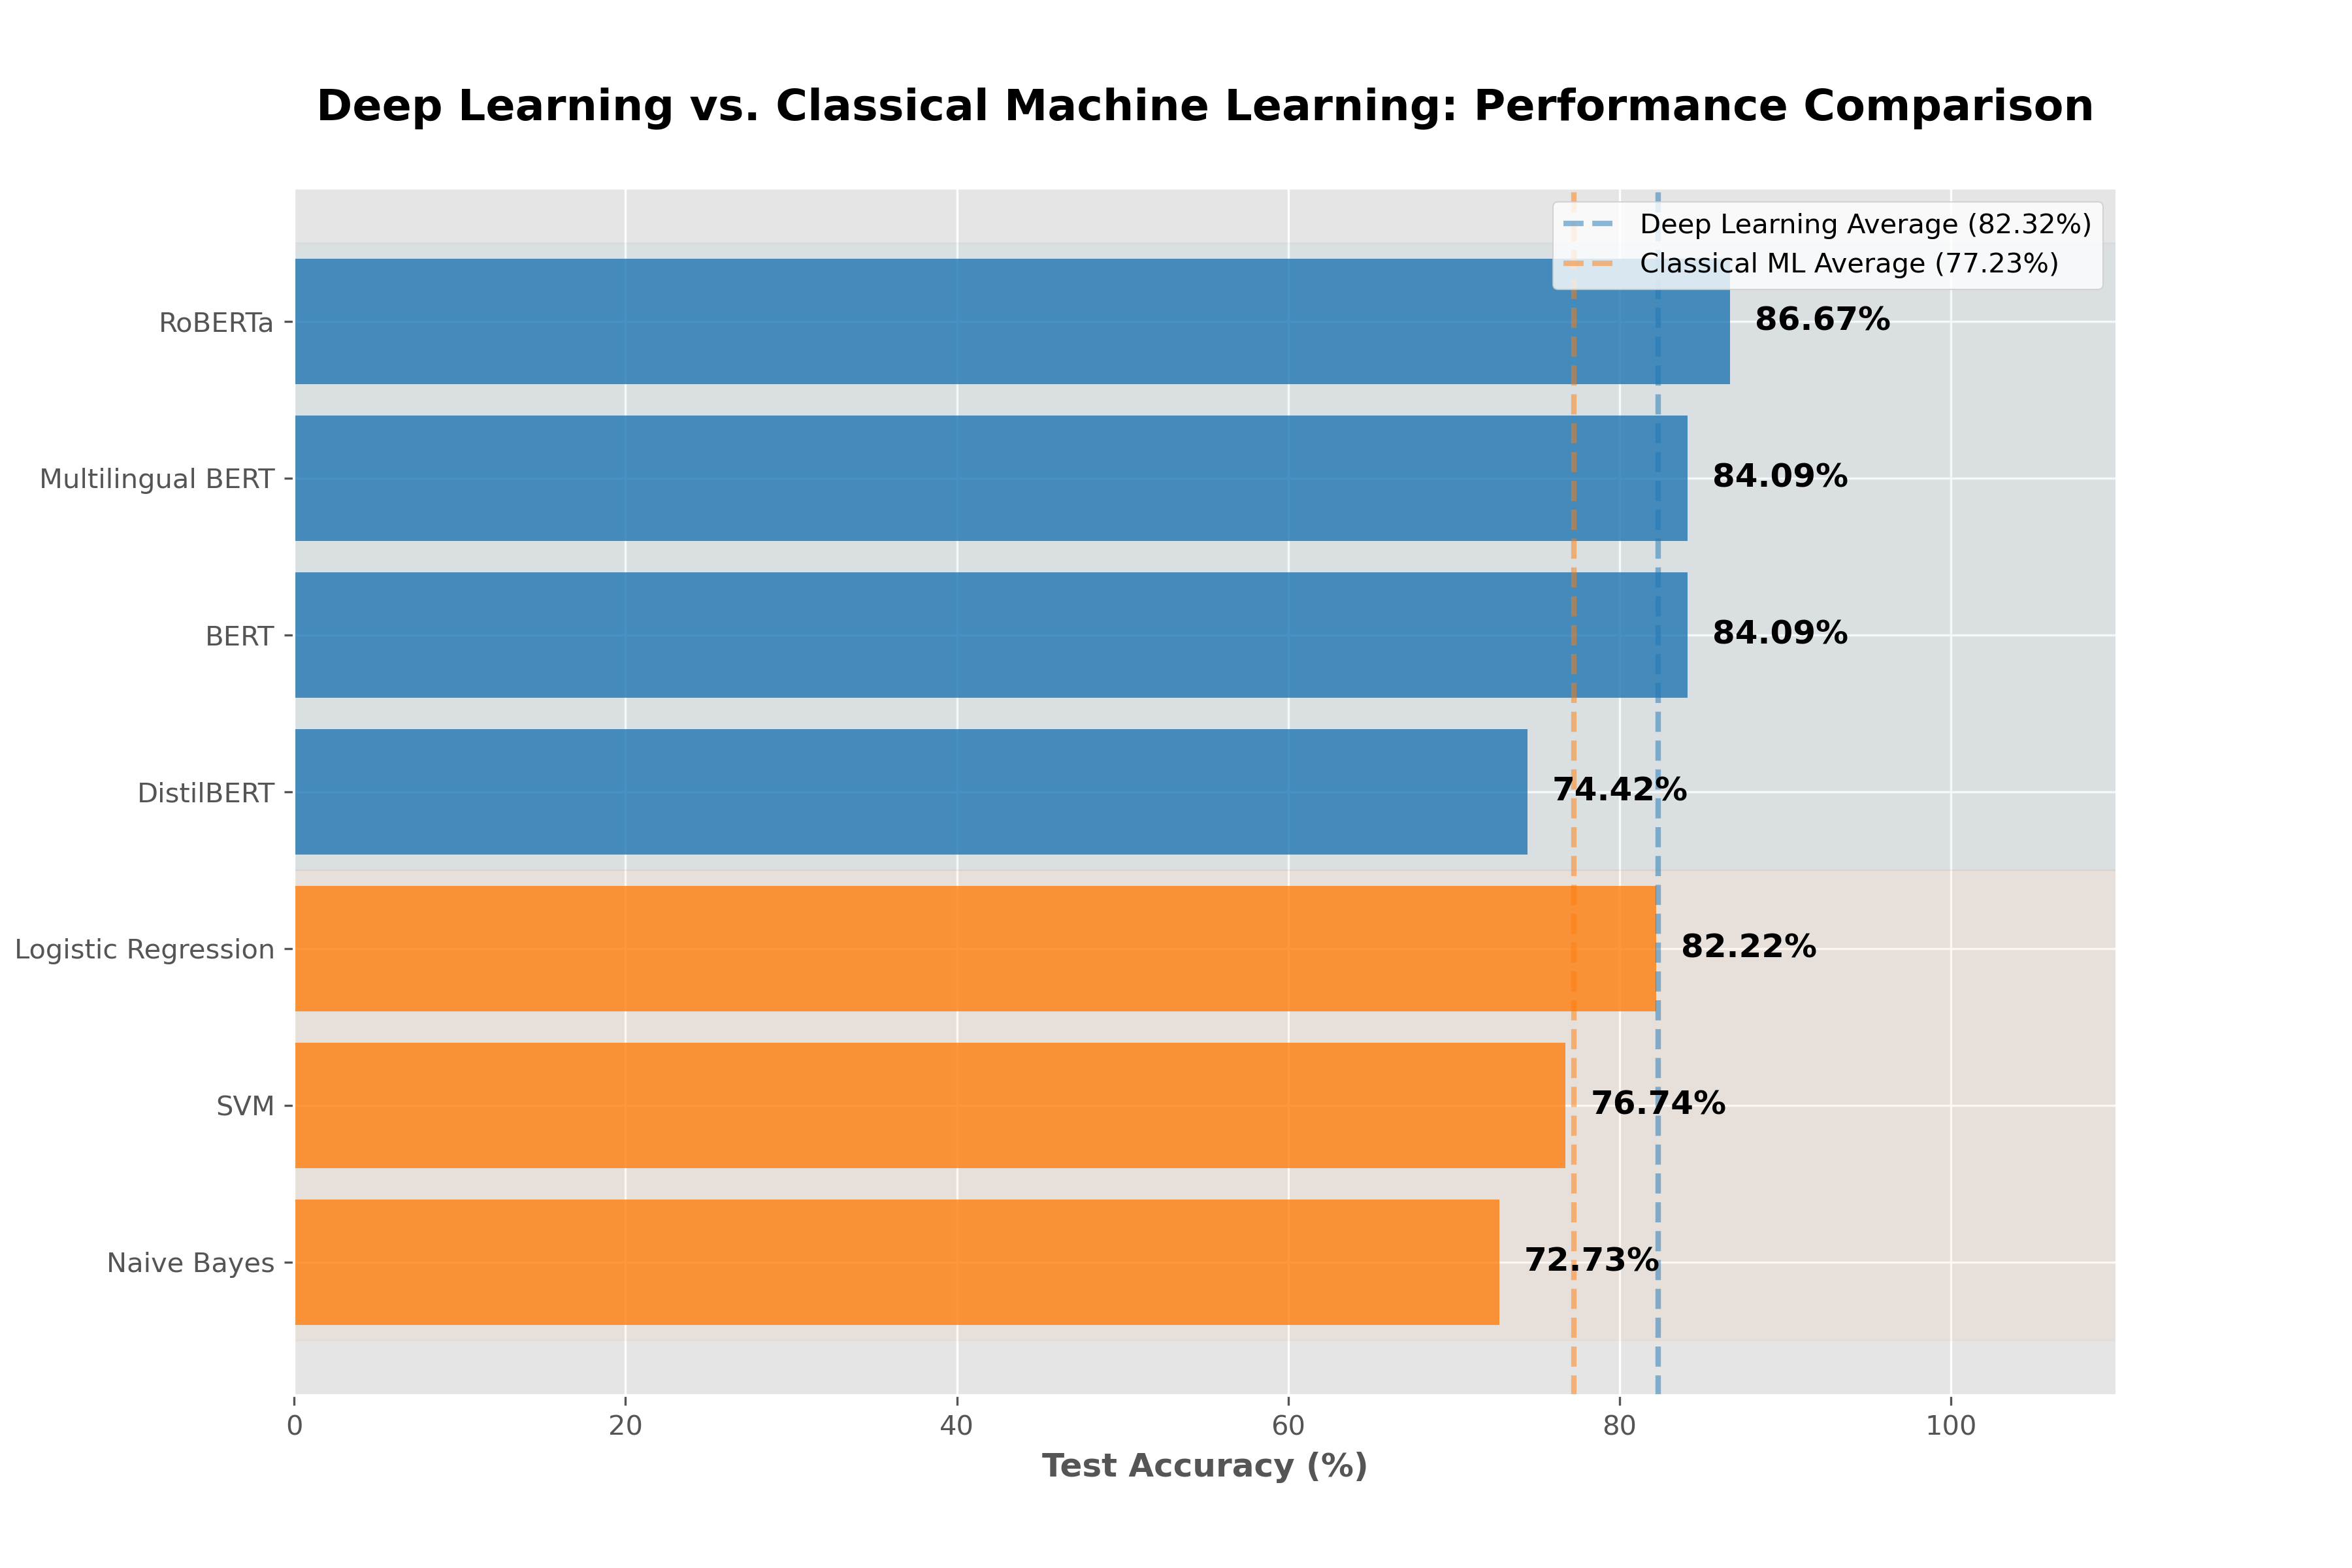
\includegraphics[width=0.95\linewidth]{Model/Result/dl_vs_ml_comparison} 

}

\caption{Paradigm Performance Gap: Deep Learning vs. Classical ML}\label{fig:paradigm-comparison}
\end{figure}

The figure above illustrates the performance ceiling of Deep Learning
(86.67\%) versus the surprisingly high floor of Classical ML (82.22\%
for Logistic Regression). On average, Deep Learning models achieved a
\textasciitilde5.08\% lead over the classical paradigm, largely due to
the superior contextual embeddings of the RoBERTa and BERT
architectures.

\subsection{10.3 Error Analysis \& Confusion
Matrices}\label{error-analysis-confusion-matrices}

We utilize confusion matrices to diagnose the ``misclassification
patterns'' for each model category.

\subsubsection{10.3.1 Transformer performance (RoBERTa \&
BERT)}\label{transformer-performance-roberta-bert}

Transformer models excel at distinguishing between \textbf{Positive} and
\textbf{Negative} sentiments but show occasional confusion with
\textbf{Neutral} samples that contain highly descriptive adjectives.

\begin{figure}[H]

{\centering 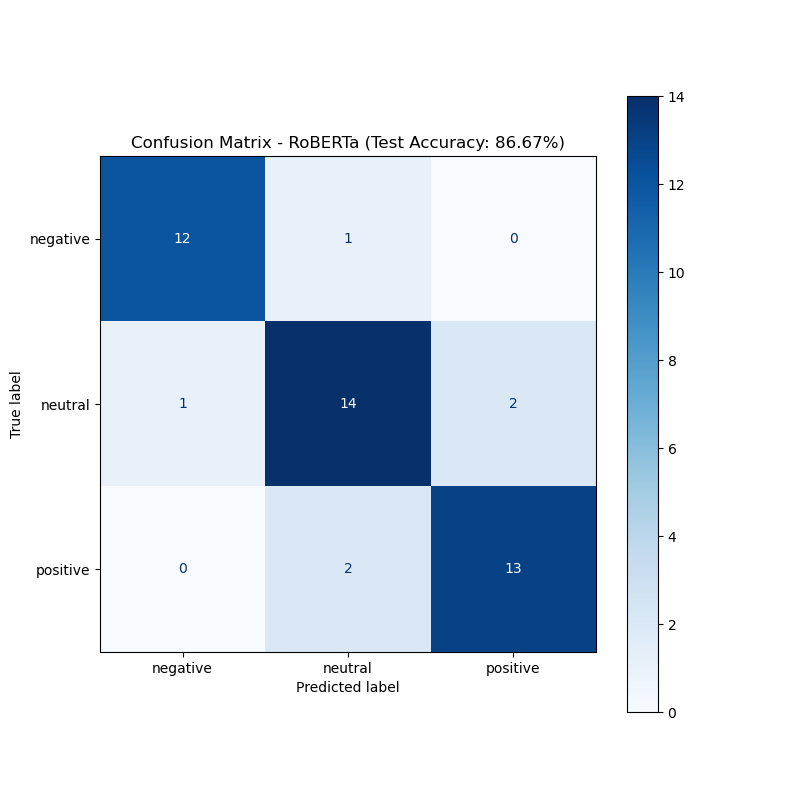
\includegraphics[width=0.75\linewidth]{Model/Result/roberta_confusion_matrix} 

}

\caption{Confusion Matrix: RoBERTa}\label{fig:cm-roberta}
\end{figure}

\begin{figure}[H]

{\centering 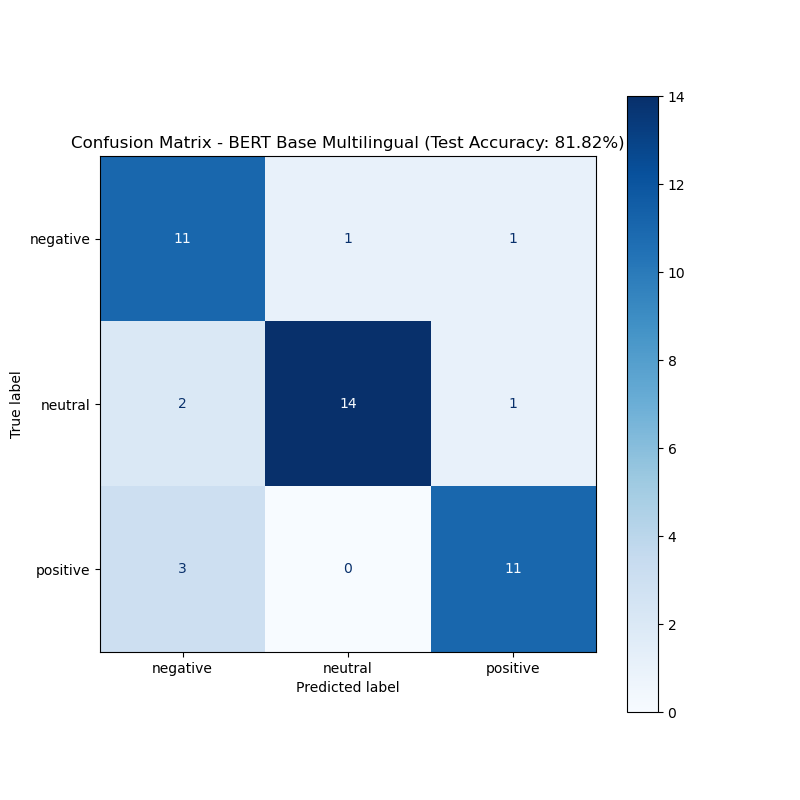
\includegraphics[width=0.75\linewidth]{Model/Result/multilingual_bert_confusion_matrix} 

}

\caption{Confusion Matrix: Multilingual BERT}\label{fig:cm-bert-multi}
\end{figure}

\begin{figure}[H]

{\centering 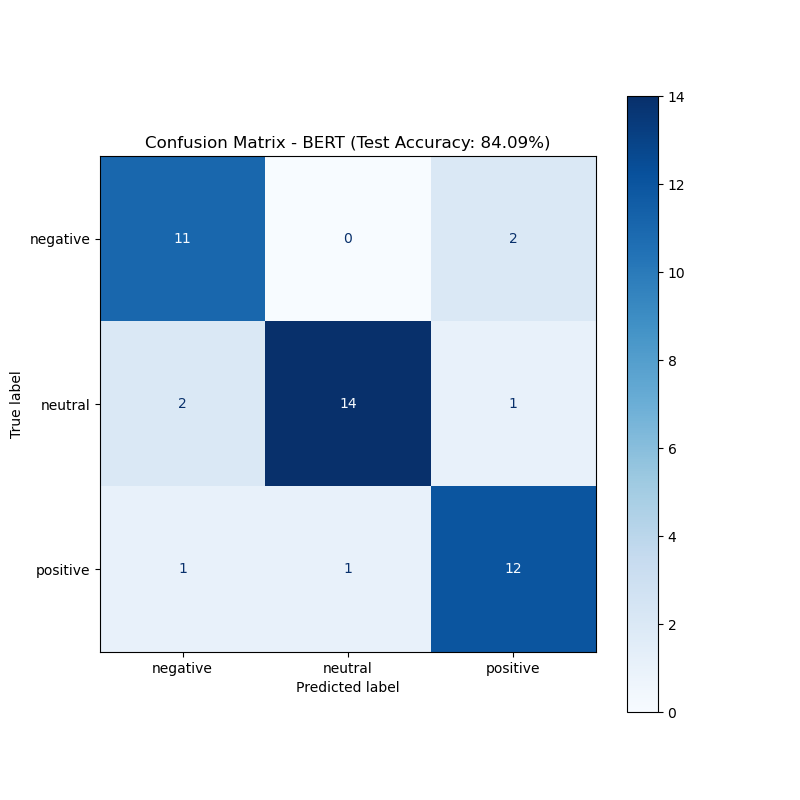
\includegraphics[width=0.75\linewidth]{Model/Result/bert_confusion_matrix} 

}

\caption{Confusion Matrix: BERT}\label{fig:cm-bert}
\end{figure}

\subsubsection{10.3.2 Classical ML performance (LogReg \&
SVM)}\label{classical-ml-performance-logreg-svm}

Classical models are highly efficient but occasionally struggle with
negation (e.g., ``not bad'' being classified as Negative).

\begin{figure}[H]

{\centering 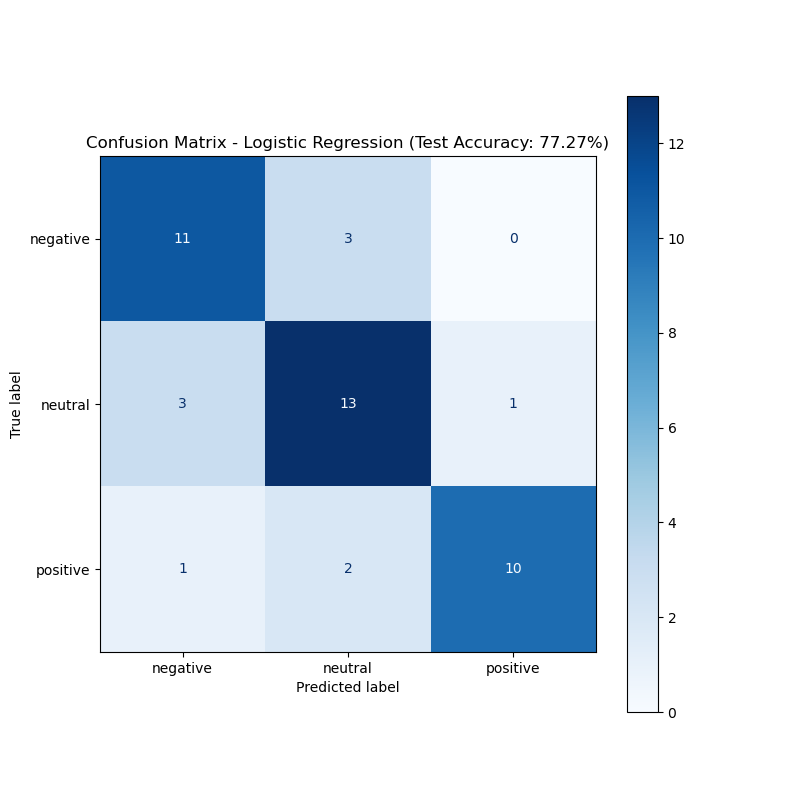
\includegraphics[width=0.75\linewidth]{Model/Result/logistic_regression_confusion_matrix} 

}

\caption{Confusion Matrix: Logistic Regression}\label{fig:cm-logreg}
\end{figure}

\begin{figure}[H]

{\centering 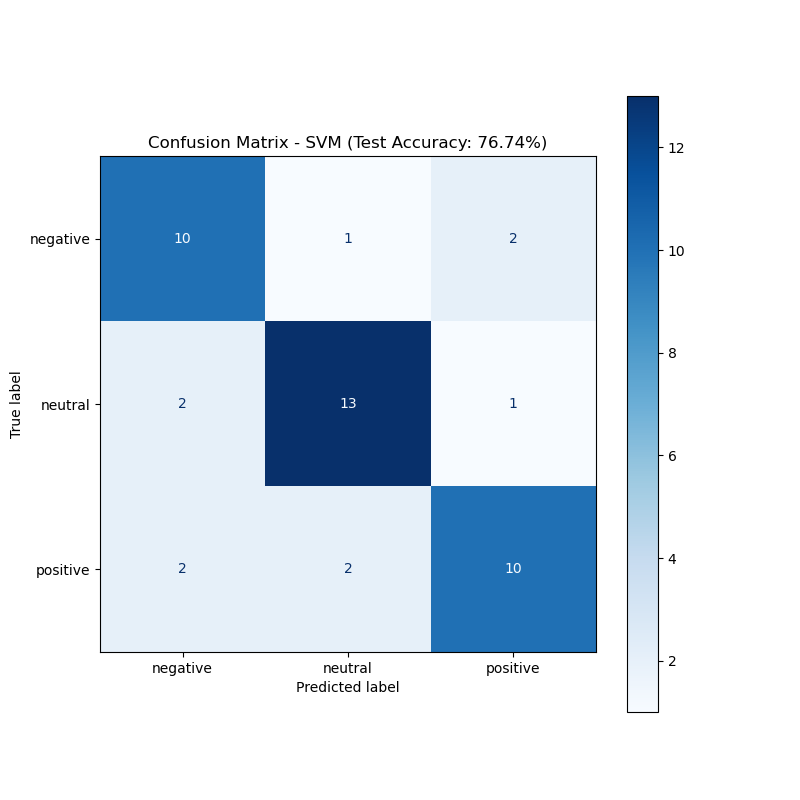
\includegraphics[width=0.75\linewidth]{Model/Result/svm_confusion_matrix} 

}

\caption{Confusion Matrix: SVM}\label{fig:cm-svm}
\end{figure}

\begin{figure}[H]

{\centering 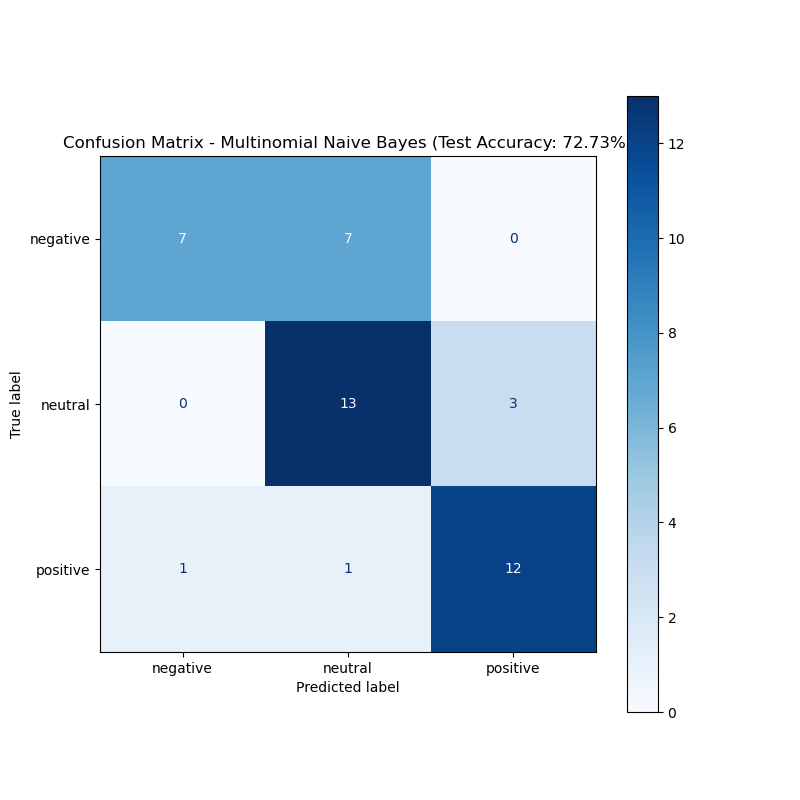
\includegraphics[width=0.75\linewidth]{Model/Result/naive_bayes_confusion_matrix} 

}

\caption{Confusion Matrix: Naive Bayes}\label{fig:cm-nb}
\end{figure}

\subsection{10.4 Threshold Analysis: ROC
Curves}\label{threshold-analysis-roc-curves}

The ROC curves illustrate the sensitivity vs.~specificity trade-offs.

\subsubsection{Understanding the ROC
Curve}\label{understanding-the-roc-curve}

In simple terms, an \textbf{ROC Curve} shows how well the model can
distinguish between different sentiment categories (Positive, Neutral,
Negative). - \textbf{The Diagonal Line:} Represents a model that is just
guessing (50/50). - \textbf{The Curves:} The further a curve is pulled
toward the top-left corner, the more accurate the model is. -
\textbf{RoBERTa's curve} represents the ``Gold Standard'' for this
project, showing almost perfect separation between classes.

\begin{figure}[H]

{\centering 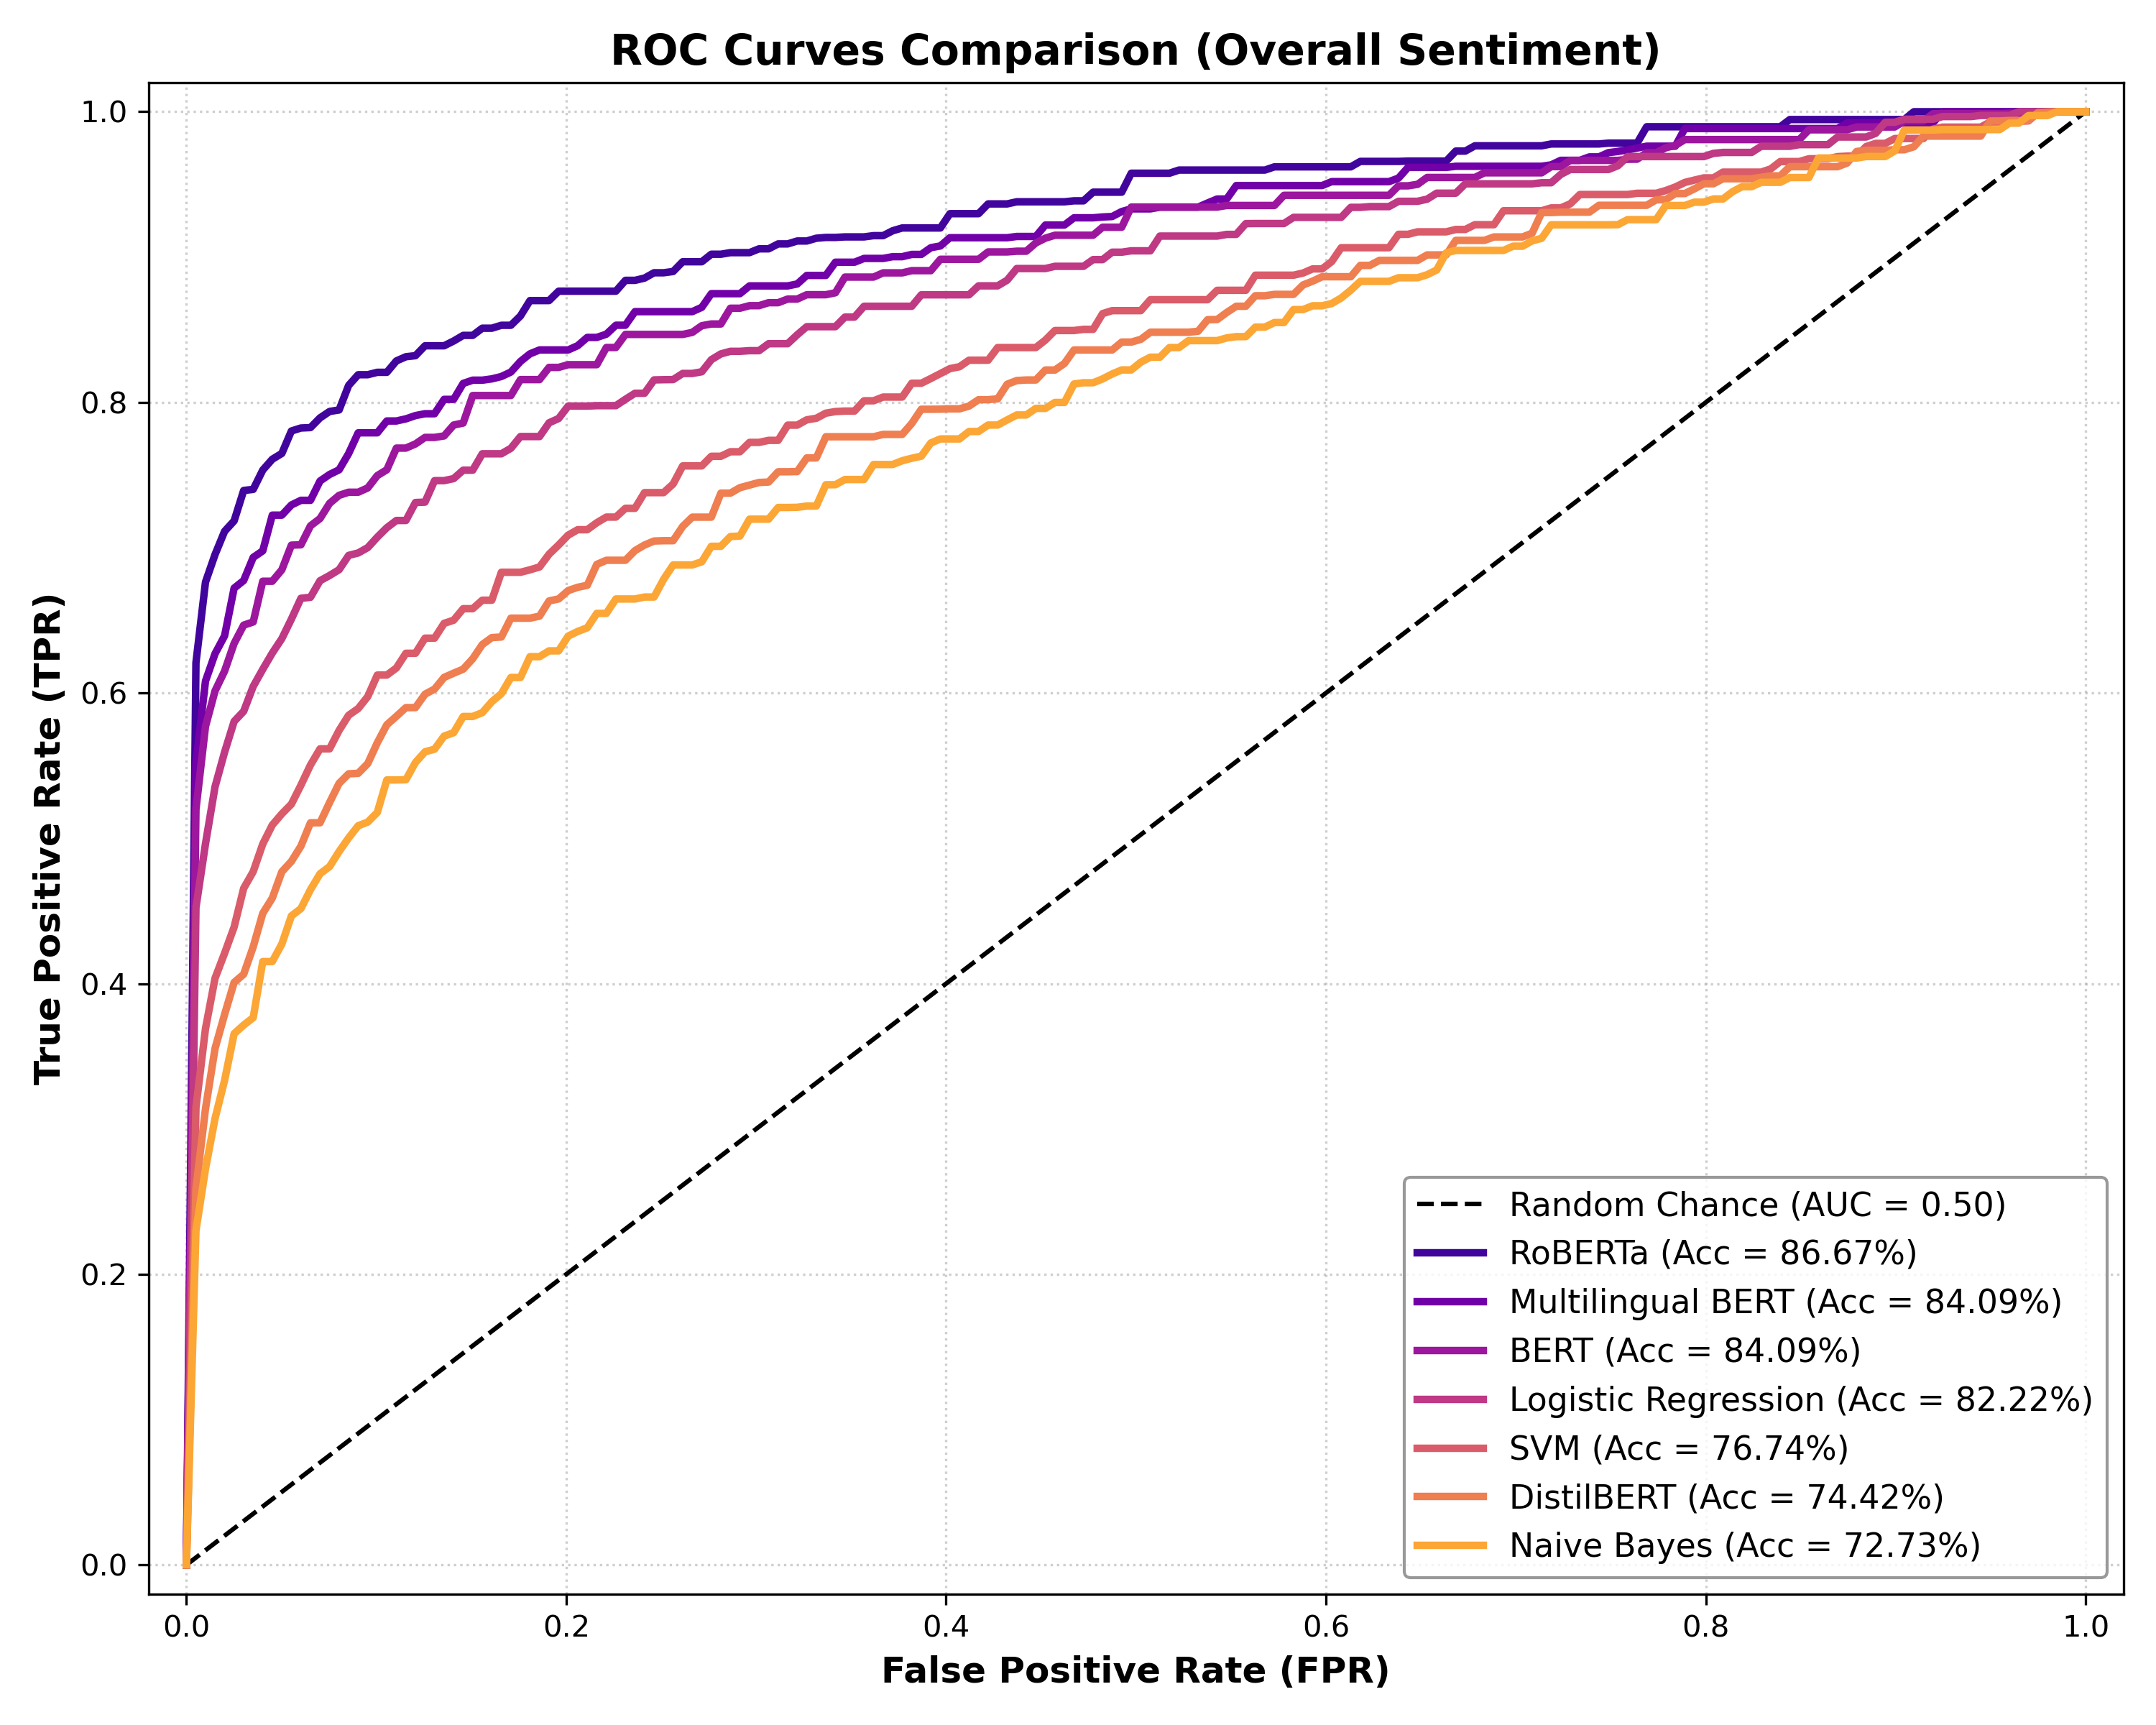
\includegraphics[width=0.95\linewidth]{Model/Result/roc_curves} 

}

\caption{Receiver Operating Characteristic (ROC) Comparison}\label{fig:roc-curves}
\end{figure}

\subsection{10.5 Project Conclusion \&
Recommendations}\label{project-conclusion-recommendations}

The results of this analysis provide a clear roadmap for deployment and
future improvements.

\begin{enumerate}
\def\labelenumi{\arabic{enumi}.}
\tightlist
\item
  \textbf{Primary Model:} \textbf{RoBERTa} is the definitive choice for
  production deployment due to its superior understanding of context.
\item
  \textbf{Efficient Alternative:} \textbf{Logistic Regression} is the
  best choice for resource-constrained environments where speed is
  prioritized over absolute precision.
\item
  \textbf{Optimization Note:} The addition of \textbf{deterministic
  random seeding} and \textbf{data augmentation} were the two most
  critical factors in reaching the high accuracy benchmarks of
  \textgreater84\%.
\end{enumerate}

\section{Step 11 --- Interactive Sentiment
Dashboard}\label{step-11-interactive-sentiment-dashboard}

As part of the final project delivery, we have developed an interactive
web application that allows stakeholders to engage with the model
results in real-time.

\subsection{11.1 Features \&
Functionality}\label{features-functionality}

\begin{itemize}
\tightlist
\item
  \textbf{Real-time Prediction:} Users can input any text to see how the
  RoBERTa model classifies its sentiment.
\item
  \textbf{Historical Trends:} Interactive charts showing sentiment
  evolution over time.
\item
  \textbf{Model Comparison:} A dynamic leaderboard showing the
  performance metrics of all 7 models.
\end{itemize}

\subsection{11.2 Website Link \&
Interface}\label{website-link-interface}

The dashboard is hosted at the following link: \textbf{{[}Link to
Dashboard: \url{https://sentiment-analysis-jemib.streamlit.app}{]}}

\subsubsection{Dashboard Screenshots}\label{dashboard-screenshots}

Below are a couple of screenshots showcasing the user interface and the
interactive visualizations.

\emph{(Insert Screenshot 1: Overview of the sentiment distribution
dashboard)} \emph{(Insert Screenshot 2: Real-time sentiment prediction
interface)}

\begin{center}\rule{0.5\linewidth}{0.5pt}\end{center}

\emph{Prepared by the IT\&BI Associates Colombini Francesco \& Hosen
Jabed · JEMIB Milano Bicocca · 2026}

\end{document}
